\documentclass[lualatex, aspectratio=169]{beamer}

\usetheme{Data61}

\title{Data Representations}
\subtitle{Text, Categories, Time Series...}
\author{Lachlan McCalman}
\institute{Inference Systems Engineering}

\usepackage{fontspec}
\usepackage{unicode-math}
\usefonttheme{serif}

\defaultfontfeatures{Ligatures=TeX}
\setmainfont{EB Garamond}
\setsansfont{Open Sans}
\setmonofont{Source Serif Pro}
\setmathfont{Asana Math}

% Math
\renewcommand{\v}[1]{\mathbf{#1}}
\renewcommand{\d}{\,\mathrm{d}}
\newcommand{\T}{^\top}
\newcommand{\vp}[1]{\mathbf{#1}^{\prime}}
\newcommand{\h}[1]{\hat{#1}}
\newcommand{\cov}[2]{\mathrm{Cov}(#1,#2)}
\newcommand{\hil}{\mathscr{H}}
\newcommand{\reals}{\mathbb{R}}
\newcommand{\complexs}{\mathbb{C}}
\newcommand{\dprod}[2]{{\langle #1, #2 \rangle}}
\newcommand{\expec}[1]{\mathbb{E}\!\left[{#1}\right]}
\newcommand{\argmin}{\operatornamewithlimits{argmin}}
\newcommand{\pd}[2]{\frac{\partial#1}{\partial#2}}
\newcommand{\norm}[1]{\|#1\|}
\newcommand{\query}[1]{{#1}^{*}}


% Text
\newcommand{\imp}[1]{\textcolor{Data61 green}{\textbf{#1}}}

%%%%%%%%%%%%%%%%%%%%%%%
% global renew commands
%%%%%%%%%%%%%%%%%%%%%%%
\makeatletter
\def\gnewcommand{\g@star@or@long\new@command}
\def\grenewcommand{\g@star@or@long\renew@command}
\def\g@star@or@long#1{% 
  \@ifstar{\let\l@ngrel@x\global#1}{\def\l@ngrel@x{\long\global}#1}}
\makeatother
%%%%%%%%%%%%%%%%%%%%%%%%%%%
% end global renew commands
%%%%%%%%%%%%%%%%%%%%%%%%%%%

\let\oldint\int
\grenewcommand\int{\oldint\!}
\grenewcommand{\epsilon}{\varepsilon}

\let\oldemptyset\emptyset
\let\emptyset\varnothing

\newtheorem{prp}{Proposition}[section]
\newtheorem{thm}{Theorem}[section]

\theoremstyle{definition}
\newtheorem{dfn}{Definition}[section]

\newcommand{\sidenote}[1]{
  \marginline{{\fontsize{8}{8}\selectfont
    \begin{spacing}{1}
#1
    \end{spacing} }}
}




# https://machinelearningmastery.com/time-series-prediction-lstm-recurrent-neural-networks-python-keras/ 
# https://blog.statsbot.co/time-series-prediction-using-recurrent-neural-networks-lstms-807fa6ca7f
# https://machinelearningmastery.com/promise-recurrent-neural-networks-time-series-forecasting/
# https://en.wikipedia.org/wiki/Dynamic_time_warping





\begin{document}

\maketitle

\begin{frame}{Similarity}
  \begin{itemize}
    \item Machine learning: Given $\{\v{X_i}, Y_i\}_{i=1}^{N}$ and $\v{X}^*$, what is $Y^*$? \\
    \item Roughly, we \emph{interpolate}: Find $\v{X}_j$ near $\v{X}^*$, then $Y^*$ is near $Y_j$
  \end{itemize}
\end{frame}

\begin{frame}{Nearest Neighbour}
  \begin{tikzpicture}[remember picture, overlay]
            \node[at=(current page.center)] {
  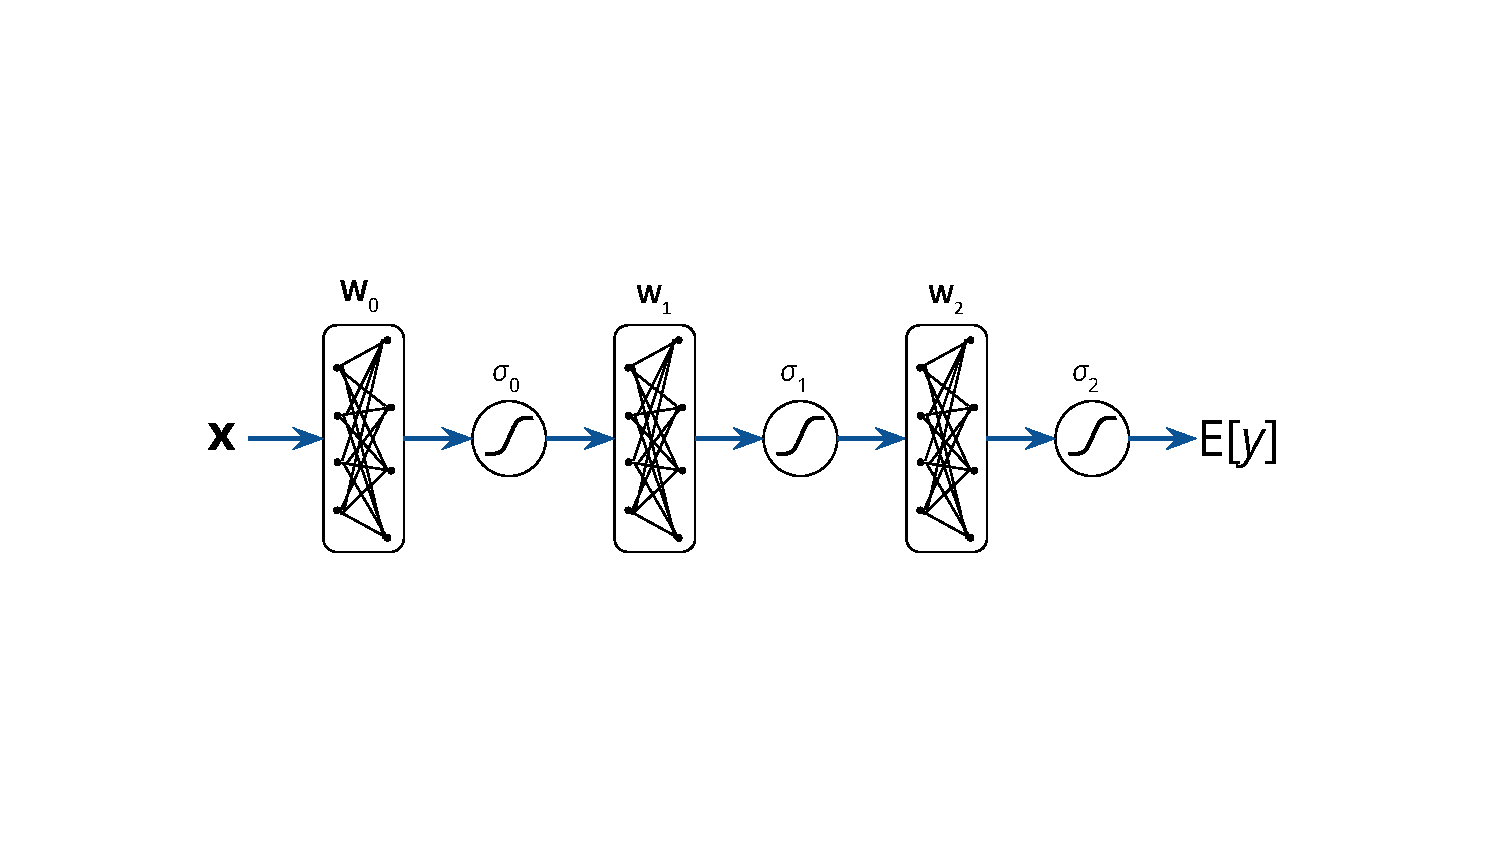
\includegraphics[page=1, width=\pagewidth]{assets/pictures.pdf}
            };
\end{tikzpicture}
\end{frame}

\begin{frame}{Parametric Model}
  \begin{tikzpicture}[remember picture, overlay]
            \node[at=(current page.center)] {
  \includegraphics[page=2, width=\pagewidth]{assets/pictures.pdf}
            };
\end{tikzpicture}
\end{frame}


\begin{frame}{What is similar?}
  \begin{itemize}
    \item But what does \alert{near} mean??
    \item We usually need some \emph{distance} function $d(\cdot, \cdot)$
    \item Different distance measures, different answers!
    \item And what if our features aren't numbers: $d(\textrm{``Apple''}, \textrm{``Pear''}) = ??$
  \end{itemize}
\end{frame}

\begin{frame}{Smooth}
  \begin{align*}
    \textrm{Given} \{X_i, Y_i\}_{i=1}^N 
  \end{align*}
\end{frame}


\begin{frame}{Difference and Similarity}
  \begin{align*}
    d((0.1, 0.3), (-0.3, 0.5)) &= \sqrt{(0.1 + 0.3)^2 + (0.3 - 0.5)^2} \\
    d(\textrm{``Apple''}, \textrm{``Pear''}) &= ??
  \end{align*}
\end{frame}

\begin{frame}{Second slide}
  \begin{enumerate}
    \item first
    \item second
    \item third
    \begin{enumerate}
      \item \alert{alert} 
      \item \structure{structure}
			\begin{enumerate}
				\item third $\Gamma\Delta\gamma$
				\item second third
			\end{enumerate}
    \end{enumerate}
  \end{enumerate}
\end{frame}


\end{document}
